\documentclass{article}
\usepackage[utf8]{inputenc}
\usepackage[icelandic]{babel}
\usepackage[T1]{fontenc}
\usepackage{graphicx}
\usepackage{mathtools}
\usepackage{amsmath}
\usepackage{amssymb}
\usepackage{minted}


\graphicspath{ {./} }
\title{Verkefni 6 - Tölv 2}
\author{ttb3@hi.is}
\date{\today}


\begin{document}
\maketitle 

\section*{2.4.5}
Ef maður setur inn lyklanna EASYQUESTION í tómt heap endar maður með YTUSQNEASIOE. Tréð myndi líta (nokkurn vegin) svona út:

\begin{tabular}{ccccccccccccccc}
    &&&&&&&Y&&&&&&&\\
    &&&T&&&&&&&&U&&&\\
    &S&&&&Q&&&&N&&&&E&\\
    A&&S&&I&&O&&E&&&&&&
\end{tabular}
% \begin{align}
%     Y&\\
%     T\quad&U\\
%     S\quad Q\quad &N\quad S\\
%     A\quad E\quad I\quad O\quad& E
% \end{align}
% \begin{center}
%     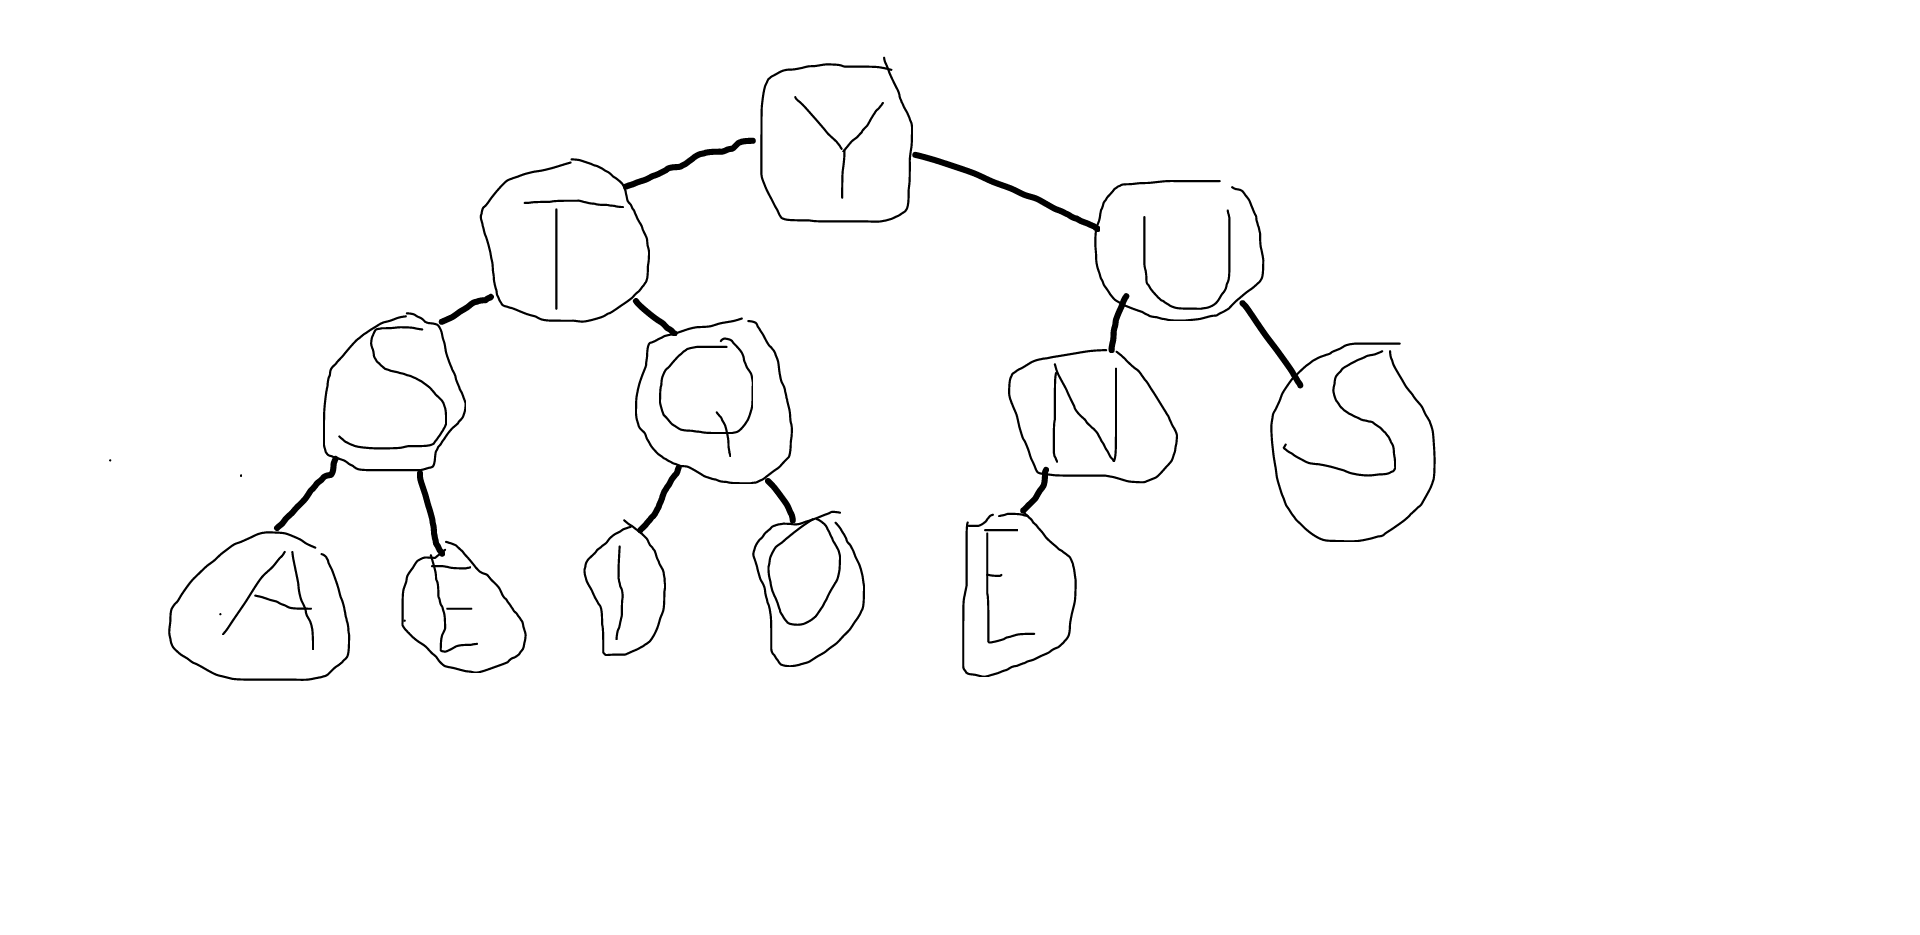
\includegraphics[scale=0.2]{Drawing.png}\\
%     betra að sjá tréð á mynd
% \end{center}

\section*{2.4.10}

% \text{Gamla númeringin er barn(i,0) = 2xi (i=1,...N), barn(i,1) = 2xi+1,foreldri(i)=i/2 f(i)=i-1 frá gömlu númerum yfir í nýju foreldri_nýja(j) = foreldri(j+1) = (j+i)/2  , j = 0...N-1 þannig svarið er að foreldri pq[k] væri (k+1)/2}

Gamla númeringin er $barn(i,0) = 2*i$ $(i=1,...N)$, $barn(i,1) = 2*i+1$ 
$foreldri(i)=\frac{i}{2}$ $f(i)=i-1$
frá gömlu númerum yfir í nýju: $foreldri_nyja(j)$ $=$ $foreldri(j+1)$ $=$ $(j+i)/2$ , $j=0...N-1$
Þannig svarið er að foreldri pq[k] væri, ef k er slétt tala: $(k-2)/2$, ef k er oddatala: $(k-1)/2$.
og til að finna barn pq[k], ef k er slétt tala: $(k*2)+2$, ef k er oddatala: $(k*2)+1$
\end{document}